\section{MultidimensionalData}
\subsection{Multi-Set Bar Charts}
I "Multi-set Bar Chart" sono grafici a barre che mostrano più insiemi di dati su uno stesso grafico, consentendo di confrontare più categorie o gruppi di dati attraverso barre separate.
In un grafico a barre tradizionale, ogni barra rappresenta un singolo insieme di dati, ad esempio una singola categoria o una serie temporale. Tuttavia, nel caso dei multi-set bar charts, diversi insiemi di dati vengono rappresentati con barre raggruppate insieme per ogni categoria o punto temporale.
Le barre per ogni categoria sono divise in sezioni separate, ognuna rappresentante un insieme di dati diverso. Questo tipo di grafico è particolarmente utile quando si desidera confrontare le relazioni tra diverse categorie attraverso più serie di dati.
Ad esempio, immagina un grafico a barre in cui ogni barra rappresenta le vendite totali mensili di diversi prodotti in un negozio. Le barre sono divise in segmenti colorati, ognuno dei quali rappresenta le vendite mensili di un prodotto specifico. Ciò consente di visualizzare facilmente le vendite totali di ogni mese e di confrontare le performance dei vari prodotti all'interno dello stesso periodo.
Questi grafici possono essere utilizzati in molteplici contesti, come analisi di mercato, confronti tra diversi gruppi di dati, analisi delle prestazioni in settori come vendite, finanza, ricerca scientifica e altro ancora.
\begin{figure}[H]
  \centering
  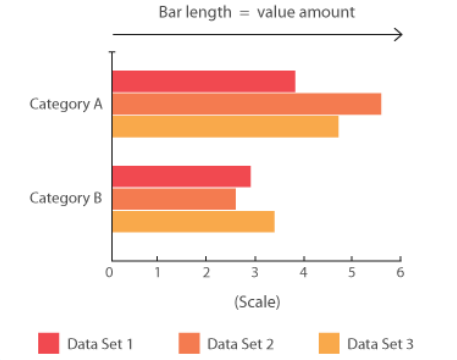
\includegraphics[width=0.5\textwidth]{images/mutiBargr.png} 
  \caption{Multi-Set Bar charts}
  \label{fig:immagine}
\end{figure}

\subsection{Multiple Bars}
Distribuzioni di ciascuna variabile tra le diverse categorie/punti dati (ogni variabile ha la propria visualizzazione).
\begin{figure}[H]
  \centering
  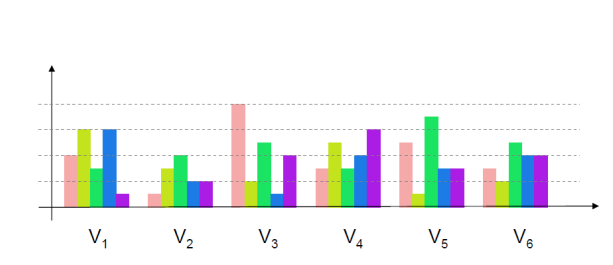
\includegraphics[width=0.5\textwidth]{images/Multiplebars.png} 
  \caption{Multiple Bars}
  \label{fig:immagine}
\end{figure}
\subsection{Stacked Bar Charts}
grafici a barre sovrapposte" o "grafici a barre impilate". Questi grafici mostrano più serie di dati sovrapposte o impilate verticalmente all'interno di ciascuna categoria o punto dati. Ogni barra rappresenta l'insieme completo dei dati per quella categoria e le diverse sezioni della barra corrispondono alle diverse componenti o sotto-categorie di quella categoria.
Simple Stacked Bar Charts:  - Utile se la visualizzazione dei valori assoluti (e la loro somma) ha significato.
Percentage Bar Charts: Migliori per mostrare le differenze relative tra le quantità nei diversi gruppi.
\begin{figure}[H]
  \centering
  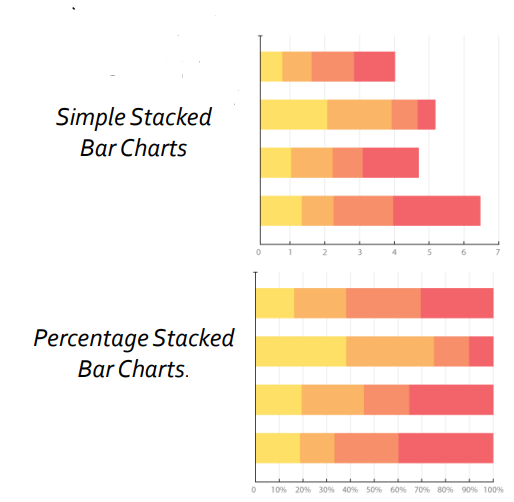
\includegraphics[width=0.5\textwidth]{images/StackedBarm.png} 
  \caption{Two types of Stacked Bar}
  \label{fig:immagine}
\end{figure}
\subsection{SpinePlots}
Gli spineplots, anche conosciuti come back-to-back plots, sono grafici utilizzati per visualizzare la distribuzione congiunta di due variabili categoriche. Questi grafici sono particolarmente utili per esaminare le relazioni tra due variabili qualitative.
La caratteristica principale degli spineplots è quella di mostrare la distribuzione incrociata delle categorie delle due variabili, disposte in modo da rivelare le associazioni tra di esse. 
\subsection{Mosaic Plots}

Un Mosaic Plot è un tipo di grafico statistico utilizzato per visualizzare la struttura relativa tra due o più variabili categoriche. Questo tipo di grafico è particolarmente utile per esaminare le relazioni tra variabili categoriche e mostrare la distribuzione proporzionale delle categorie in modo visivo.
\textbf{Vantaggi}:
\begin{itemize}
  \item Massimo utilizzo dello spazio disponibile
  \item Buona panoramica delle proporzioni tra i dati
  \item Buona panoramica della dipendenza delle variabili
\end{itemize}

\textbf{Svantaggi}:
\begin{itemize}
  \item È difficile estendere il grafico a molte variabili
\end{itemize}
\begin{figure}[H]
  \centering
  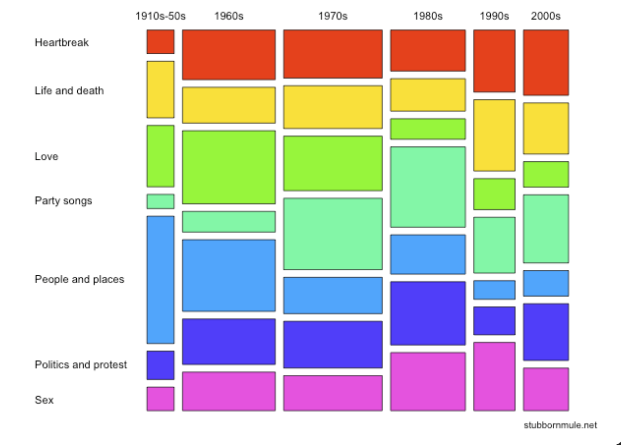
\includegraphics[width=0.5\textwidth]{images/MosaicPlots.png} 
  \caption{Mosaic Plots}
  \label{fig:immagine}
\end{figure}
\subsection{Tree Maps}
Un modo alternativo per visualizzare una struttura dati ad albero.
Efficiente nello spazio (!)
Il modo in cui i rettangoli sono divisi e ordinati in sottorettangoli dipende dall'algoritmo di suddivisione utilizzato.
\begin{figure}[H]
  \centering
  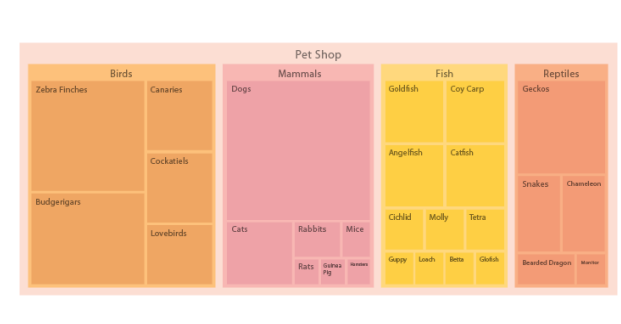
\includegraphics[width=0.5\textwidth]{images/TreeMaps.png} 
  \caption{Mosaic Plots}
  \label{fig:immagine}
\end{figure}
\subsection{Parallel Coordinates}


\textbf{Parallel Coordinates} è una tecnica di visualizzazione che consente di rappresentare graficamente relazioni complesse tra molteplici variabili. È utilizzato principalmente per esplorare e visualizzare dataset multivariati
\begin{figure}[H]
  \centering
  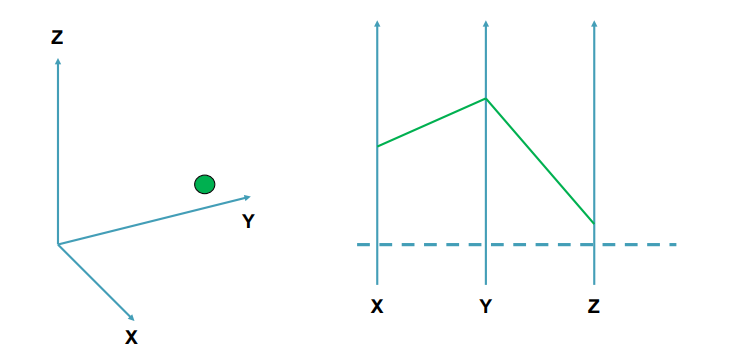
\includegraphics[width=0.5\textwidth]{images/Parallelcord.png} 
  \caption{Mosaic Plots}
  \label{fig:immagine}
\end{figure}
\subsection{Star Plot}
Conosciuto con molti nomi: grafico radar, grafico a ragnatela, grafico a rete, ecc.
Analogamente alle coordinate parallele, ma gli assi sono posizionati in coordinate polari (equi-angolari).
La posizione del primo asse non fornisce informazioni rilevanti.
Facile per confrontare le proprietà di una classe di oggetti o di una categoria.
Non è facile comprendere il compromesso tra diverse variabili.
Non adatto a molte variabili o a molti dati.
\begin{figure}[H]
  \centering
  \includegraphics[width=0.5\textwidth]{images/Starplot.png} 
  \caption{Star Plot}
  \label{fig:immagine}
\end{figure}